\documentclass[14pt,a4paper]{article}
\usepackage{mathtools}
\usepackage{amsmath}
\setcounter{MaxMatrixCols}{20}
\usepackage{setspace}
\usepackage{amsfonts}
\usepackage{graphicx}
\usepackage{geometry}
\geometry{a4paper, total = {210mm,297mm},left=35mm, right=25mm,top=25mm,bottom=25mm}
\usepackage{xcolor}
\usepackage[24pt]{mcode}
\usepackage{listings}
\lstset{basicstyle = \fontsize{12}{13} \selectfont\ttfamily}

%Begin document - Final Project ME5554 - Applied Linear Systems

\begin{document}
\label{cover}
\begin{center}
	\vspace*{3cm}
	\large{\textbf{ME-5554 Applied Linear System \\ Final Project}}
	\vfill
	\textbf{Luan Cong Doan} \\ luandoan@vt.edu
	\vfill
	Dec 7, 2015
\end{center}
\pagebreak

The design engineer at Precision 3D Measuring Inc. have just developed a prototype 3D Coordinate Measuring Machine (CMM). In order to keep the cost low, the engineers have significantly reduced the amount of structural support in the frame, which unfortunately increase the compliance at the measurement probe. High compliance is generally not acceptable in a precision measurement system.\\

\begin{figure} [htp]
	\centering
	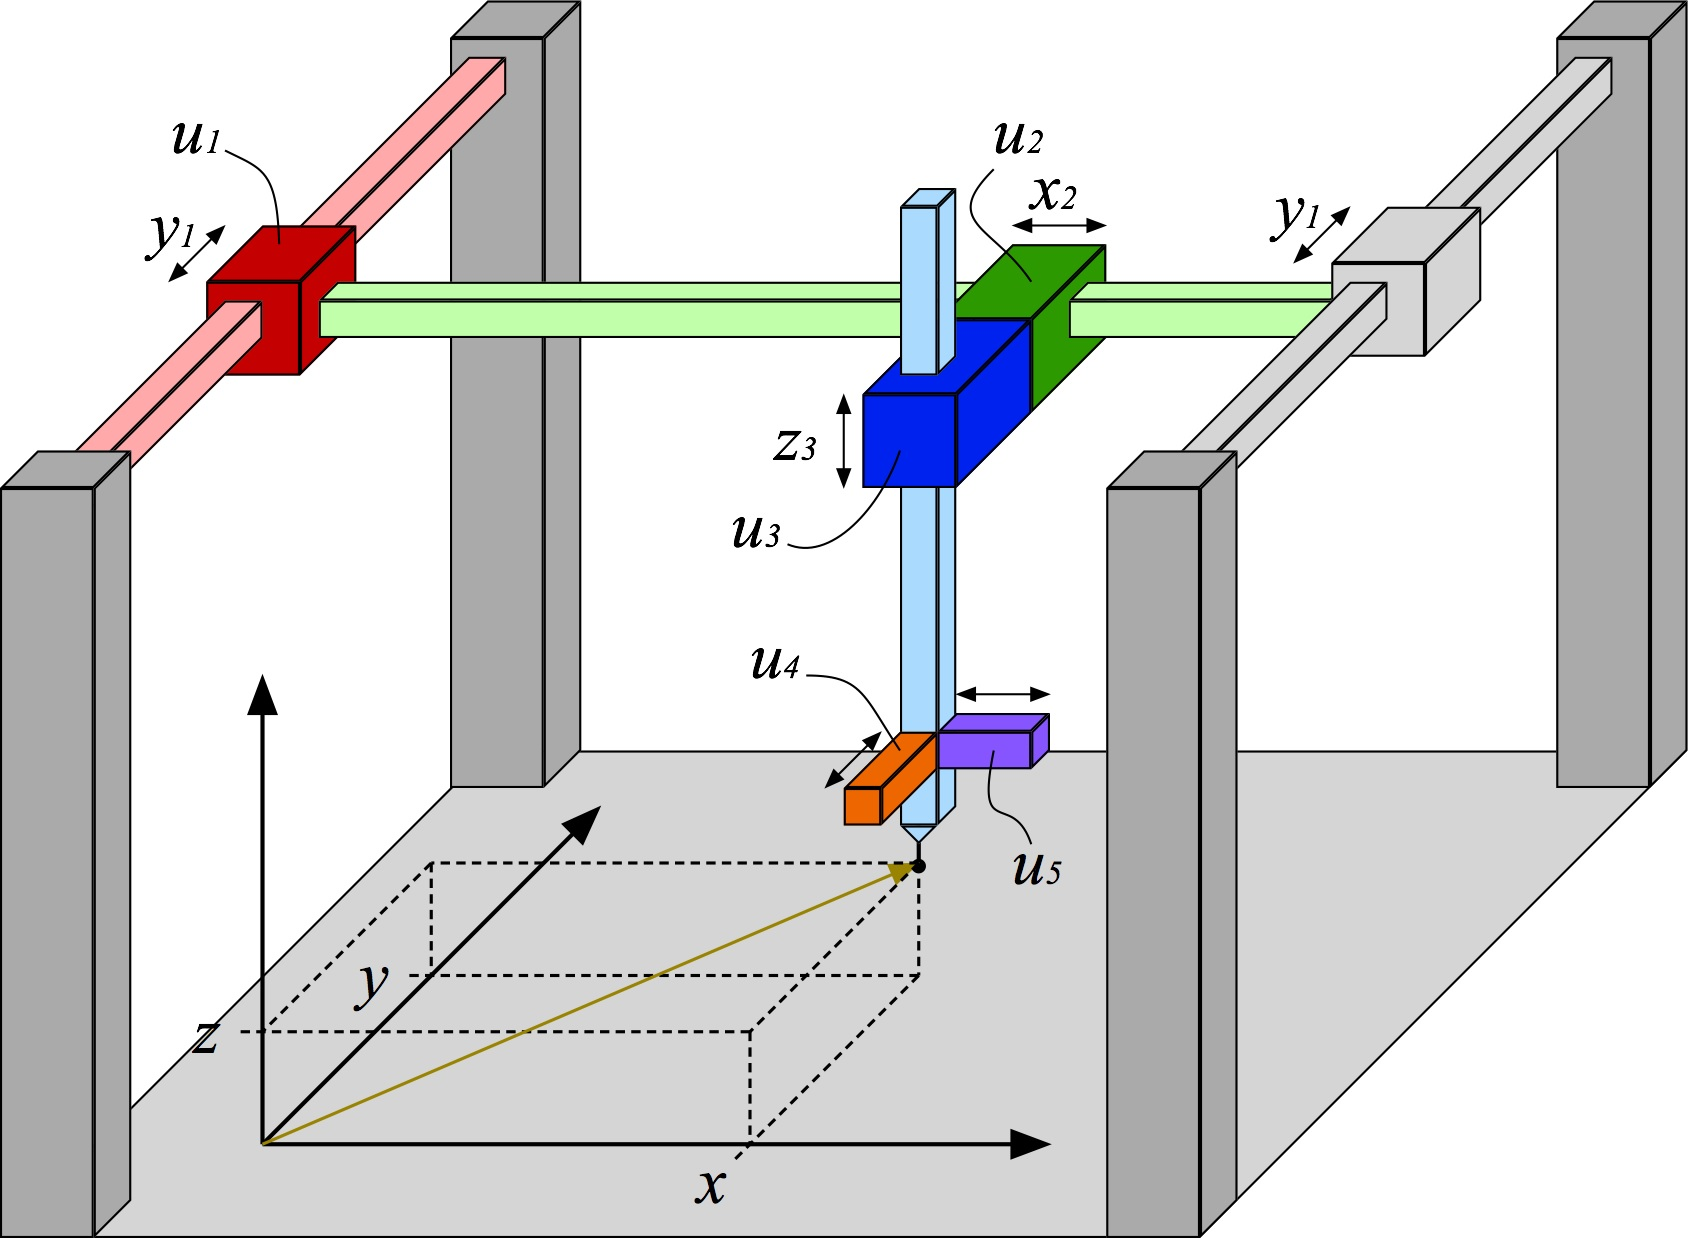
\includegraphics[scale=0.4]{MidtermProject.jpg}
	\caption{Prototype 3D Coordinate Measurement System}
\end{figure}

\large\textbf{Equation of Motion}\\
	The equation of motion for prototype CMM have already been derived and are given by the following equations:\\
	\doublespacing
	$ \hspace*{1cm} \dot{p}_1 = \alpha_1u_1 - \left(\dfrac{b_y}{M_y}\right)p_1 - \dot{p}_4   \hspace{3cm}  \dot{p}_5 = \alpha_2u_2 - \left(\dfrac{b_x}{M_x}\right)p_5 - \dot{p}_8 \\$
	$ \hspace*{1cm} \dot{q}_2 = \left(\dfrac{1}{M_y}\right)p_1 - \left(\dfrac{1}{m_4}\right)p_4 - \dot{q}_3   \hspace{2.2cm}  \dot{q}_6 = \left(\dfrac{1}{M_x}\right)p_5 - \left(\dfrac{1}{m_5}\right)p_8 - \dot{q}_7 $\\
	$ \hspace*{1cm} \dot{q}_3 = \left(\dfrac{1}{b_4}\right)\left(\alpha_4u_4 + \dot{p}_4 - k_4q_3\right)    \hspace{2.5cm}  \dot{q}_7 = \left(\dfrac{1}{b_5}\right)\left(\alpha_5u_5 + \dot{p}_8 - k_5q_7\right)$\\
	$ \hspace*{1cm} \dot{p}_4 = k_yq_2    \hspace{6.2cm}  \dot{p}_8 = k_xq_6 $\\
	$ \hspace*{1cm} \dot{y}_1 = \left(\dfrac{1}{M_y}\right)p_1    \hspace{5.2cm} \dot{x}_2 = \left(\dfrac{1}{M_x}\right)p_5 $\\
	$\hspace*{1cm} y = y_1 - q_2   \hspace{5.9cm} x = x_2 - q_6 $\\
	$ \hspace*{1cm} M_z\ddot{z} = -b_z\dot{z} + \alpha_3u_3 \\$

\pagebreak

\label{Problems}
\doublespacing
	Because the final project only focus on the y-direction dynamics, states and control signals. So we have:\\
	\textbf{State Space is defined:} \\
	\hspace*{5cm}	$\dot{S}_y = A_y.S_y + B_y.u_y \\
	\hspace*{5.2cm}		y = C_y.S_y + D_y.u_y $ \\
	With: \\
	\textbf{State variables:}  $S_y = {\begin{bmatrix} y_1&p_1&q_2&q_3&p_4 \end{bmatrix}}^T $ \\
	\hspace*{3.3cm} $\dot{S}_y = {\begin{bmatrix} \dot{y}_1 & \dot{p}_1 & \dot{q}_2 &\dot{q}_3 & \dot{p}_4 \end{bmatrix}}^T $ \\
	\textbf{Input:} $ u_y = \begin{bmatrix} u_1 \\ u_4 \end{bmatrix} $ \\
	State matrix:\\
	\hspace*{2cm} $ A_y = \begin{bmatrix} 0& \dfrac{1}{M_y} & 0&0&0 \\ 0& -\dfrac{b_y}{M_y} & -k_y&0&0 \\ 0& \dfrac{1}{M_y} & -\dfrac{k_y}{b_4} & \dfrac{k_4}{b_4} & -\dfrac{1}{m_4} \\ 0&0& \dfrac{k_y}{b_4} & -\dfrac{k_4}{b_4} &0 \\ 0&0& k_y &0&0 \end{bmatrix}$ \\
	Input matrix: \\
	\hspace*{2cm} $ B_y = \begin{bmatrix} 0&0 \\ \alpha_1 &0 \\ 0& -\dfrac{\alpha_4}{b_4} \\ 0& \dfrac{\alpha_4}{b_4} \\ 0&0 \end{bmatrix} $\\
	Output matrix: \hspace{1cm}	$ C_y = \begin{bmatrix} 1& 0& -1& 0& 0 \end{bmatrix} $ \\
	Direct Transmission matrix: $ D_y = [0]$ \\ 
	Numerical values: \\
	$ M_y = 150 kg, \hspace{0.3cm}     M_x = 100 kg,  \hspace{0.3cm}   M_z = 50 kg,  \hspace{0.3cm}   b_y = 40 Ns/m,  \hspace{0.3cm}   b_x = 50 Ns/m, \\
	b_z = 10 Ns/m, \hspace{0.3cm}  k_x = 0.2 N/m,  \hspace{0.3cm}  m_4 = 20 kg,  \hspace{0.3cm}  b_4 = 2.51 Ns/m, \hspace{0.3cm} k_4 = 7.89 N/m, \\
	m_5 = 20 kg, \hspace{0.3cm} b_5 = 3.77 Ns/m, \hspace{0.3cm} k-5 = 7.89 N/m, \hspace{0.3cm} k_y = 0.1 N/m, \\
	\alpha_1 = 0.05 N/V, \hspace{0.3cm} \alpha_2 = 0.1 N/V,  \hspace{0.3cm} \alpha_3 = 0.1 N/V,  \hspace{0.3cm} \alpha_4 = 0.3 N/V, \hspace{0.3cm} \alpha_5 = 0.5 N/V $ \\
	\pagebreak
	
	So we have numerical results: \\
	State matrix $A_y$: \\
	\hspace*{2.5cm} $ A_y = \begin{bmatrix} 0& 0.0067 & 0&0&0 \\ 0 & -0.2667 & -0.1 &0&0\\ 0& 0.0067 & -0.0398 & 3.1434 & -0.05\\ 0&0& 0.0398 & -3.1434 &0 \\ 0&0 & 0.1 &0&0 \end{bmatrix} $ \\
	
	Input matrix $B_y$: \\
	\hspace*{2.5cm} $ B_y = \begin{bmatrix} 0&0 \\ 0.05 &0 \\ 0& -0.1195 \\ 0& 0.1195 \\ 0&0 \end{bmatrix}$  \\
	
	Output matrix $C_y$: \\
	\hspace*{2.5cm}$ C_y = \begin{bmatrix} 1 0 -1 0 0 \end{bmatrix} $ \\
	
	Direct Transmission matrix $D_y$: $D_y = [0]$ \\
	
\pagebreak

\large\textbf{Problem 1:} Determine the observability of the open-loop plant.\\
	Matlab code:
	\begin{lstlisting}
		Ob = obsv(A_y,C_y)';   % observability of system check
		rOb = rank(Ob);
		testO = size(A_y,1);
		fprintf('Rank of observability matrix is %d. ', rOb);
		if rOb == testO
		fprintf('System is observable.\n');
		else
		fprintf('System is not observable.\n');
		end
	\end{lstlisting}
	Result:
	\begin{lstlisting}
		Rank of observable matrix is 5. System is observable.
	\end{lstlisting}

\vspace{1cm}
\large\textbf{Problem 2:} Design the state feedback controller gains with conditions: \\
% requirement
\hspace*{2cm} $ |y| \leq 0.2 m $ after 10 seconds \\
\hspace*{2cm} $ |u_1| \leq 10000, \hspace{1.5cm} |u_4| \leq 1000 $\\
\hspace*{2cm} $ y_1(0) = 0.2; \hspace{1.5cm} p_4(0) = -0.5 , $ \hspace{1.5cm} all other states are zero.\\
	Matlab code:
	\begin{lstlisting}
	SF0 = [0.2; 0; 0; 0; -0.5]; % initial condition for problem 2
	CPoles = [linspace(-1.1, -1.0,5)];     % poles location
	G = place(A_y,B_y,CPoles);
	AcF = A_y - B_y*G;
	BF = [];
	syscF = ss(AcF, BF, C_y,D_y);
	
	[ycF,tcF,xcF] = initial(syscF,SF0,16);
	figure;	plot(tcF,ycF(:,1));
	grid on; 
	xlabel('Time'); ylabel('Output y-direction');
	title('Output of Y in 16 seconds');
	print('OutputYdirection16s','-dpng');
	
	U = -G*xcF';
	figure;	plot(tcF,U(1,:),'r',tcF,U(2,:),'b');
	grid on; legend('u1','u4');  
	xlabel('Time'); ylabel('Control response');
	title('Control input space for U1 and U4 in 16 seconds');
	print('ControlInputU1U4_16s','-dpng');
	\end{lstlisting} 
	
	Ouput in Y direction:
	\begin{figure}[htp]
		\begin{center}
			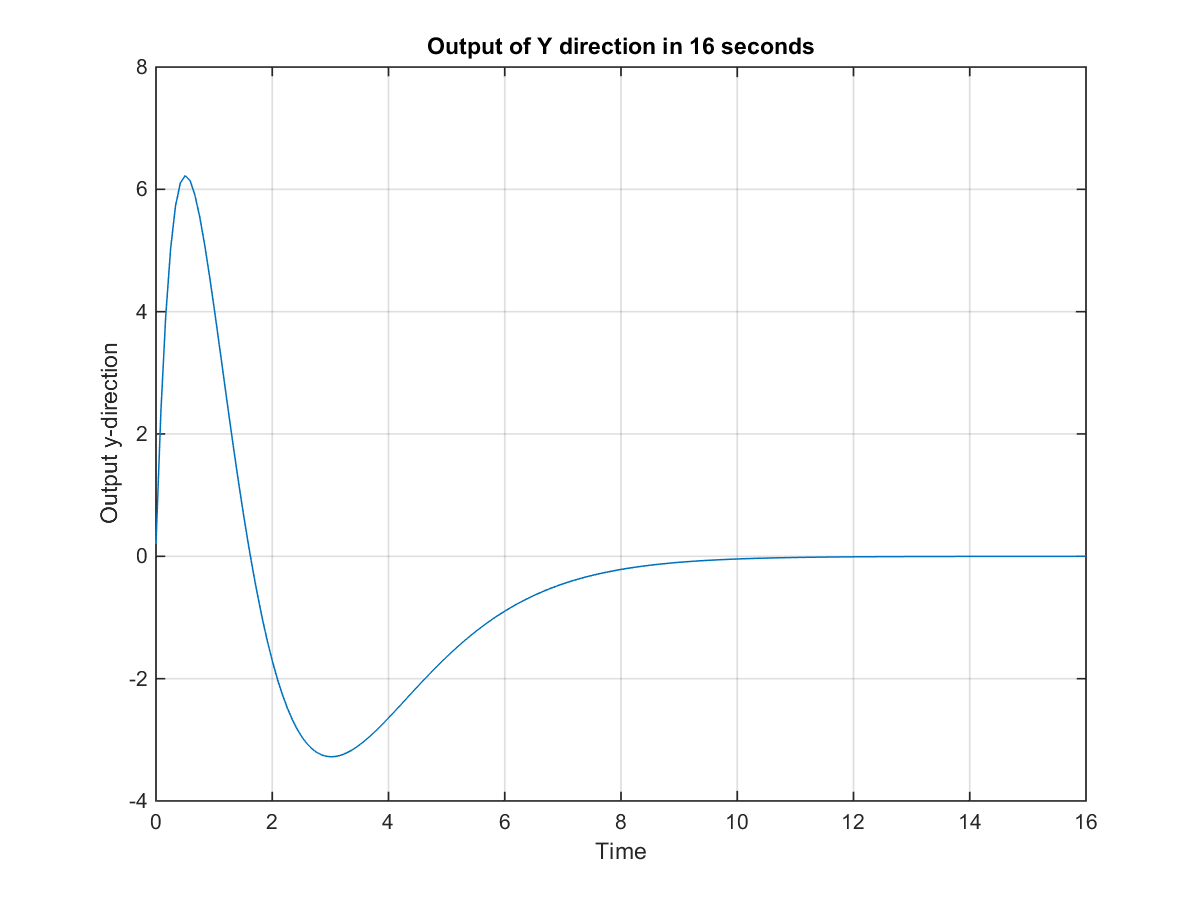
\includegraphics[scale=0.8]{OutputYdirection16s.png}
			\caption{Output in Y direction in 16s}
		\end{center}
	\end{figure}
	\pagebreak
	
	Control input space of U1 and U4:
	\begin{figure}[htp]
		\begin{center}
			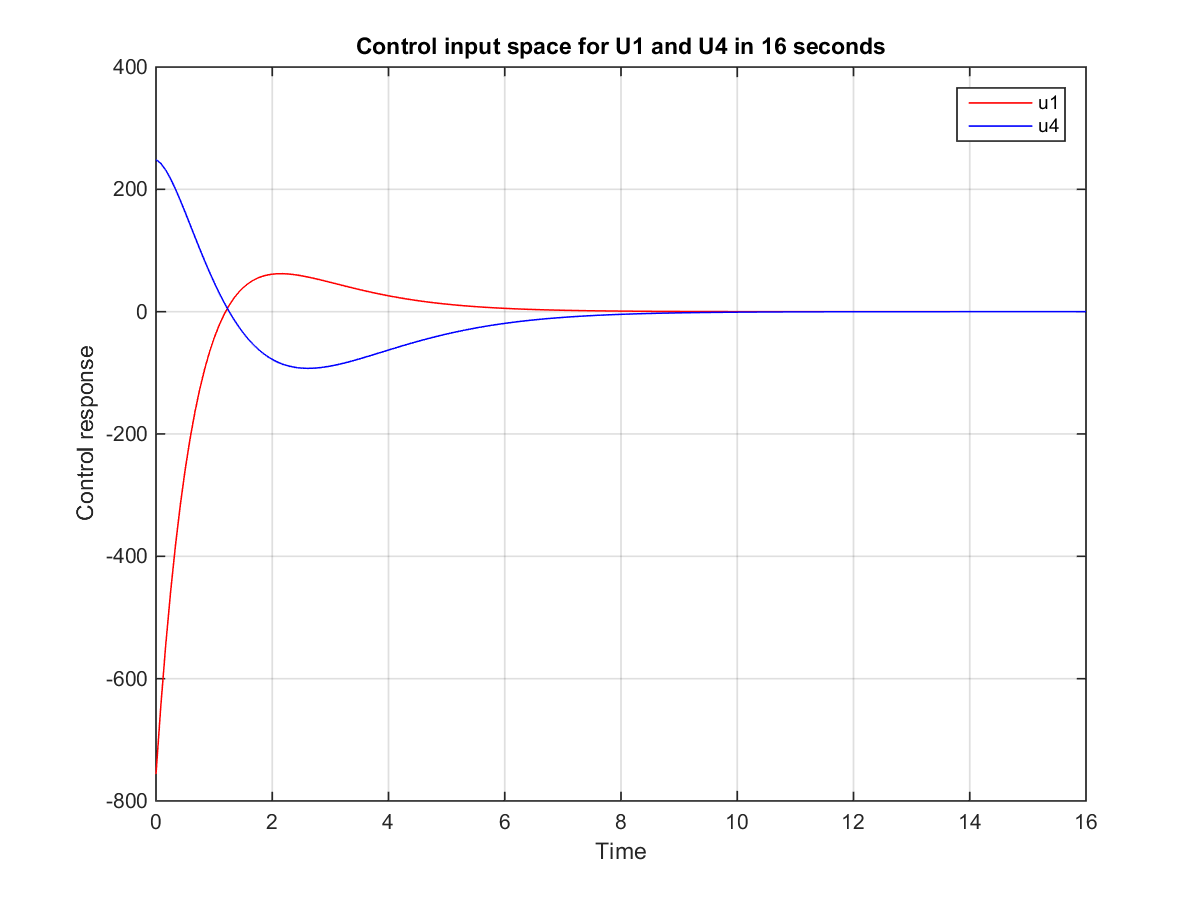
\includegraphics[scale=0.8]{ControlInputU1U4_16s.png}
			\caption{Control input of U1 and U4 in 16s}
		\end{center}
	\end{figure}
	
	The state feedback controller gains $G$ is:
	\begin{lstlisting}
	G
	
	G =
	
	1.0e+03 *
	
	3.9346    0.0367   -0.6439   -0.6449    0.0618
	-1.9330   -0.0001    1.9068    1.9065   -0.2761
	\end{lstlisting}
	
	\pagebreak

\large\textbf{Design closed-loop estimation:} \\
	State-space equation: \hspace{1cm}	$\dot{S}_y = A_y.S_y + B_y.u_y \\
	\hspace*{5.3cm}		y = C_y.S_y + D_y.u_y $ \\
	with $K$ is the observer feedback matrix we have Dynamic State Estimator:\\
	\hspace*{2cm} $ \dot{\hat{S}}_y = \hat{A}_y\hat{S}_y + \hat{B}_yu_y + K(y - \hat{y}) \\
	\hspace*{2.3cm} \hat{y} = \hat{C}_y\hat{S}_y + \hat{D}_y.u_y $ \\
	with assume that we have a perfect model: $ A_y = \hat{A}_y, \hspace{0.5cm} B_y = \hat{B}_y \\ \hspace*{8cm} C_y = \hat{C}_y, \hspace{0.5cm} D = \hat{D} $ \\
	Poles for closed-loop observer: \\
	\hspace*{2cm} $ OPoles = \begin{bmatrix} -8&-6.5&-5& -0.5& 0 \end{bmatrix}$ \\
	
	Open-loop poles, closed-loop poles and the observer poles: 
		\begin{figure}[htp]
			\begin{center}
				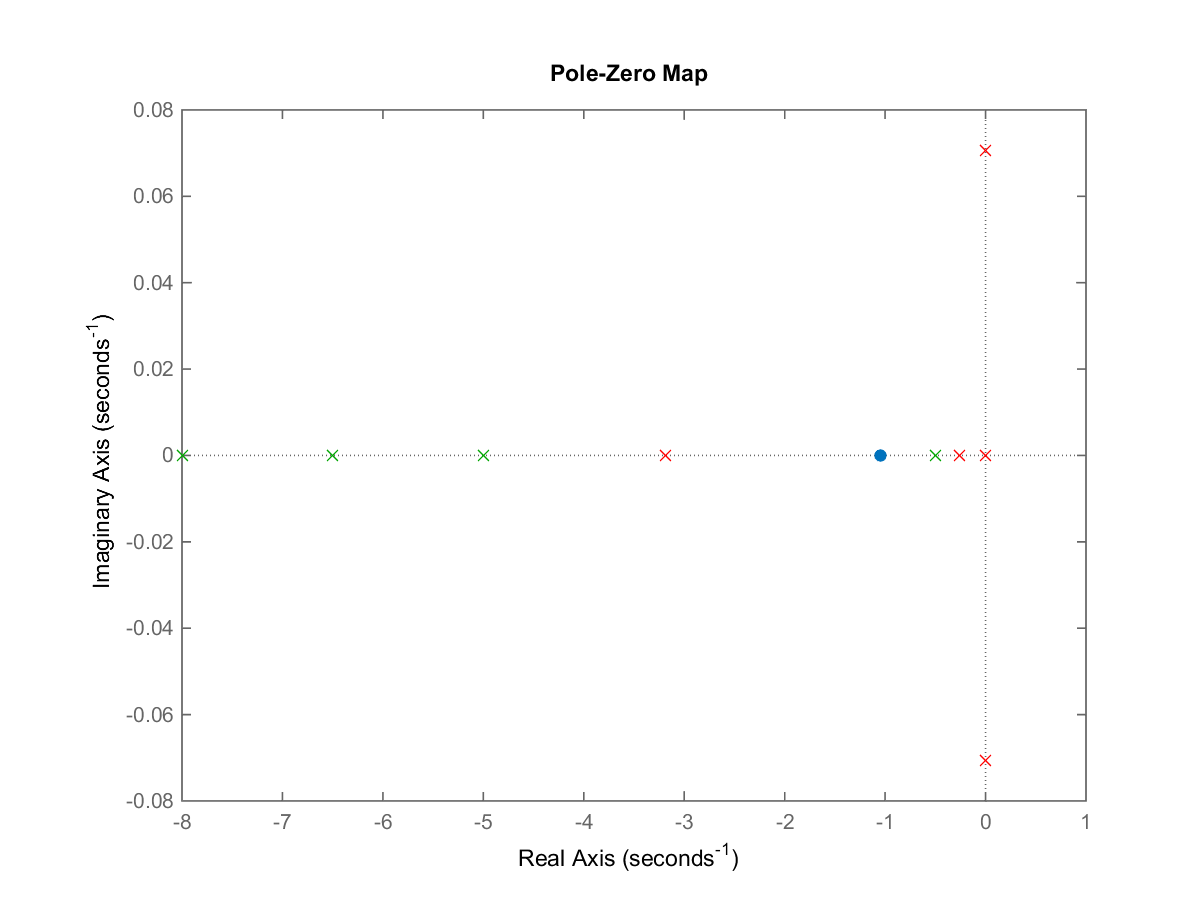
\includegraphics[scale = 0.7]{PolesPlot.png}
				\caption{Open-loop poles, closed-loop poles, and observer poles}
			\end{center}
		\end{figure} \\
	red x - poles for Open-loop system. green x - poles for observer system. \\
	blue circle - poles for closed-loop (because 5 poles very close together, so it support to be like a circle on pole-zero map).	
	\pagebreak
	
	The state estimation error dynamics for the Luenberger observer is defined: \\
	\hspace*{2cm} $ e_y = S_y - \hat{S}_y \Rightarrow \dot{e}_y = \dot{S}_y - \dot{\hat{S}}_y $ \\
	Output estimation error: $ \tilde{y} = y - \hat{y} $ \\
	We have the state estimation error dynamics: \hspace{0.5cm} $ \dot{e}_y(t) = [A_y - KC_y]e_y(t) $ \\
	\hspace*{9cm} $ \tilde{y} = C_ye_y(t) $ \\
	The first 4 seconds should be an open loop response of the plant to allow the observer to converge, and the controller cannot be turned on until 4 seconds. It means that observer out put $\tilde{y}$ should reduced to 0 in first 4 seconds. \\
	We have this solved by Matlab: 
	\begin{lstlisting}
	OPoles = [-8 -6.5 -5 -0.5 0];  % poles for closed-loop observer
	Ob0 = [0; 0; 0; 0; 0];         % initial condition of observer
	e0 = S0 - Ob0;                 % initial for error estimation
	K = place(A_y',C_y',OPoles)';
	% Check error estimate
		AoE = A_y - K*C_y;
		BoE = [];
		CoE = C_y;
		DoE = [];
	sysOE = ss(AoE, BoE, CoE, DoE);     % system oberver error
	[yOE, tOE, sOE] = initial(sysOE, e0, 16);
	figure;
	plot(tOE,yOE); grid on;
	xlabel('Time'); ylabel('Error estimation');
	title('Error Estimation by Observation');
	print('ErrorEstimation','-dpng');
	\end{lstlisting}
	\pagebreak
	
	Result: 
		\begin{figure}[htp]
			\begin{center}
				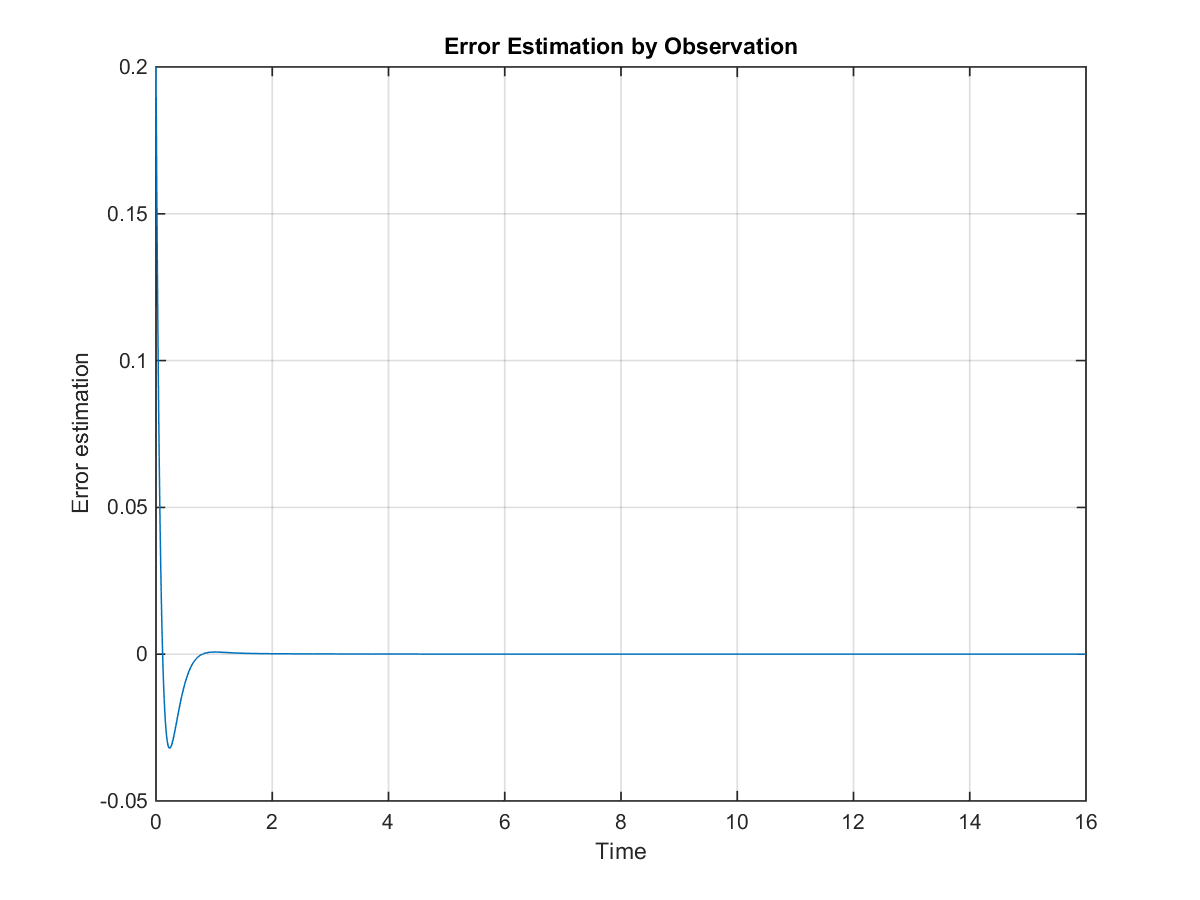
\includegraphics[scale = 0.8]{ErrorEstimation.png}
				\caption{Error estimation in 16 seconds}
			\end{center}
		\end{figure} \\
	
	For first 4 seconds, system should be an open-loop response of the plant to allow the observer to converge. So we have first augmented state-space system for open-loop and observer: \\
	\hspace*{2cm} $ \begin{bmatrix} \dot{S}_y \\ \dot{\hat{S}}_y \end{bmatrix} = \begin{bmatrix} A_y &0 \\ KC_y& A_y - KC_y \end{bmatrix}\begin{bmatrix} S_y \\ \hat{S}_y \end{bmatrix} + \begin{bmatrix} B_y \\ B_y  \end{bmatrix}u $\\
	
	\hspace*{1.8cm} $\begin{bmatrix} y\\ \hat{y} \end{bmatrix} = \begin{bmatrix} C_y&0 \\ 0&C_y \end{bmatrix}\begin{bmatrix} S_y \\ \hat{S}_y \end{bmatrix} $ \\
	
	The augmented system has twice as many states and outputs as the plant or observer. So we have: \\
\begin{lstlisting}
Zero1 = zeros(5,5);  Zero2 = zeros(1,5); % create temp zero matrix
Ag0 = [0.2;0;0;0;-0.5;0;0;0;0;0];  % initial condition for Augmented
G2 = [G,G];               % gain for Augmented
Ag = [A_y, Zero1; K*C_y, A_y-K*C_y];
Bg = [B_y; B_y];
Cg = [C_y, Zero2; Zero2, C_y];
Dg = [];
sysOp = ss(Ag, Bg, Cg, Dg);
[yOp, tOp, sOp] = initial(sysOp, Ag0, 4);
figure;
plot(tOp, yOp(:,1),'r', tOp, yOp(:,2),'--'); grid on;
xlabel('Time'); ylabel('Output open-loop and observation');
legend('Open-loop','Oservation');
title('Open-loop Plant with Observation');
print('OpenLoopObservation','-dpng');
\end{lstlisting}
	Result: 
	\begin{figure}[htp]
		\begin{center}
			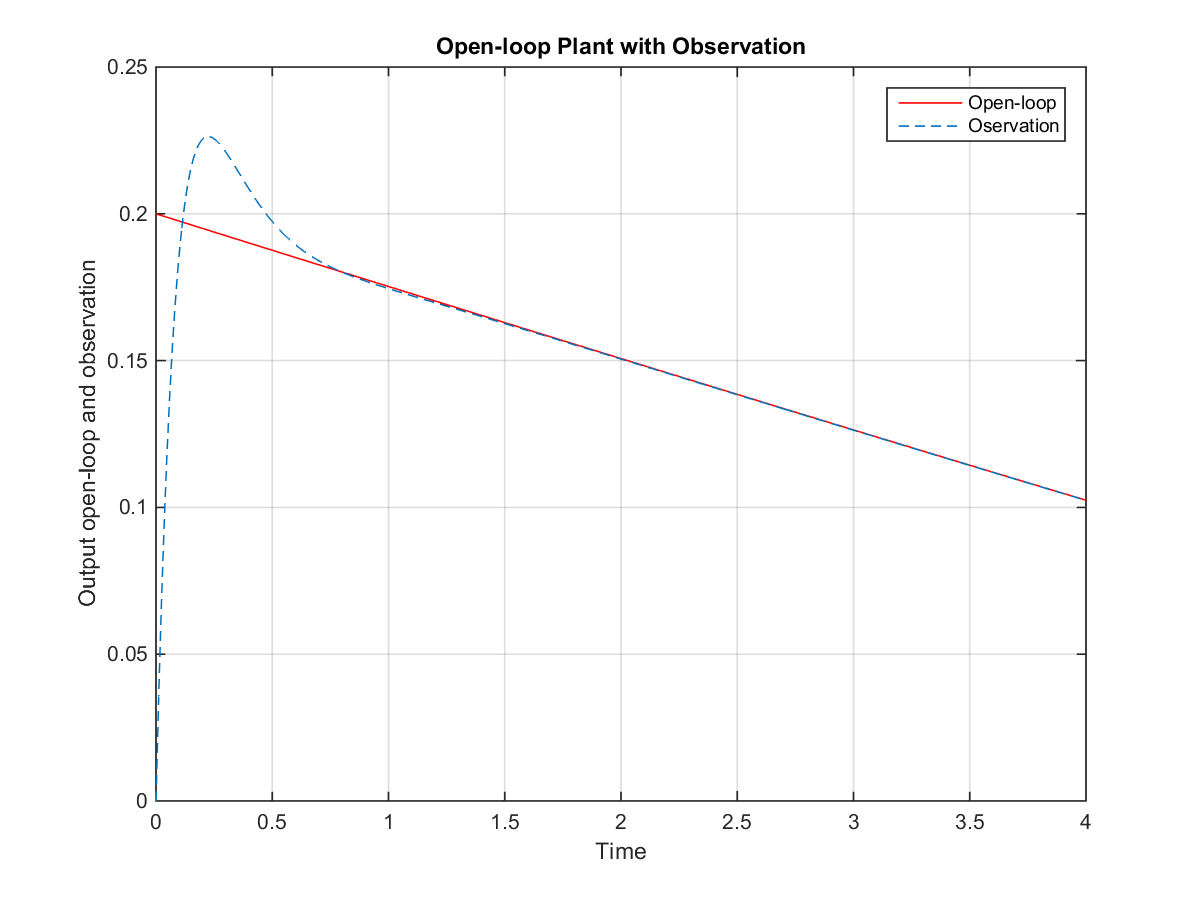
\includegraphics[scale = 0.7]{OpenLoopObservation.png}
			\caption{Open-loop Observation in first 4 seconds}
		\end{center}
	\end{figure}
	\pagebreak
	
	After 4 seconds, controller will be turned on, we will have the full state feedback control law with: \\
	- Estimated states: \hspace{1cm} $ u_y = - G.\hat{S}_y $ \\
	- Initial condition is the latest state of above Open-loop and observation system: \\ \hspace*{4.6cm} $ int0 = sOp(end,:) $ \\
	The augmented state space of full state feedback system is defined: \\
	\hspace*{2cm} $ \begin{bmatrix} \dot{S}_y \\ \dot{\hat{S}}_y \end{bmatrix} = \begin{bmatrix} A_y &-B_yG \\ KC_y& A_y - KC_y - B_yG \end{bmatrix}\begin{bmatrix} S_y \\ \hat{S}_y \end{bmatrix} + [0]u'$ \\
	
	\hspace*{1.8cm}$ \begin{bmatrix} y\\ \hat{y} \end{bmatrix} = \begin{bmatrix} C_y&0 \\ 0&C_y \end{bmatrix}\begin{bmatrix} S_y \\ \hat{S}_y \end{bmatrix} + [0]u'$ \\ 
	
	Solving system by Matlab:
\begin{lstlisting}
AgC = [A_y, -B_y*G; K*C_y, A_y-K*C_y-B_y*G];
BgC = [];
CgC = [C_y, Zero2; Zero2, C_y];
DgC = [];
int0 = sOp(end,:);
sysOC = ss(AgC, BgC, CgC, DgC);
[yOC, tOC, sOC] = initial(sysOC, int0, 12);
figure;
plot(tOC, yOC(:,1),'r', tOC, yOC(:,2), '--'); grid on;
xlabel('Time'); ylabel('Observation output');
legend('Closed-loop','Oservation');
title('Closed-loop Plant with Observation');
print('ClosedLoopObservation','-dpng');

UgC = -G2*sOC';
figure; plot(tOC, UgC); grid on;
xlabel('Time'); ylabel('Control input'); legend('u1','u4');
title('Control inputs Close-loop Observation');
print('ClosedLoopControlInput','-dpng');
\end{lstlisting}
\pagebreak

Output in Y-direction and Control Inputs of closed-loop observation simulation: 
\begin{figure}[htp]
	\begin{center}
		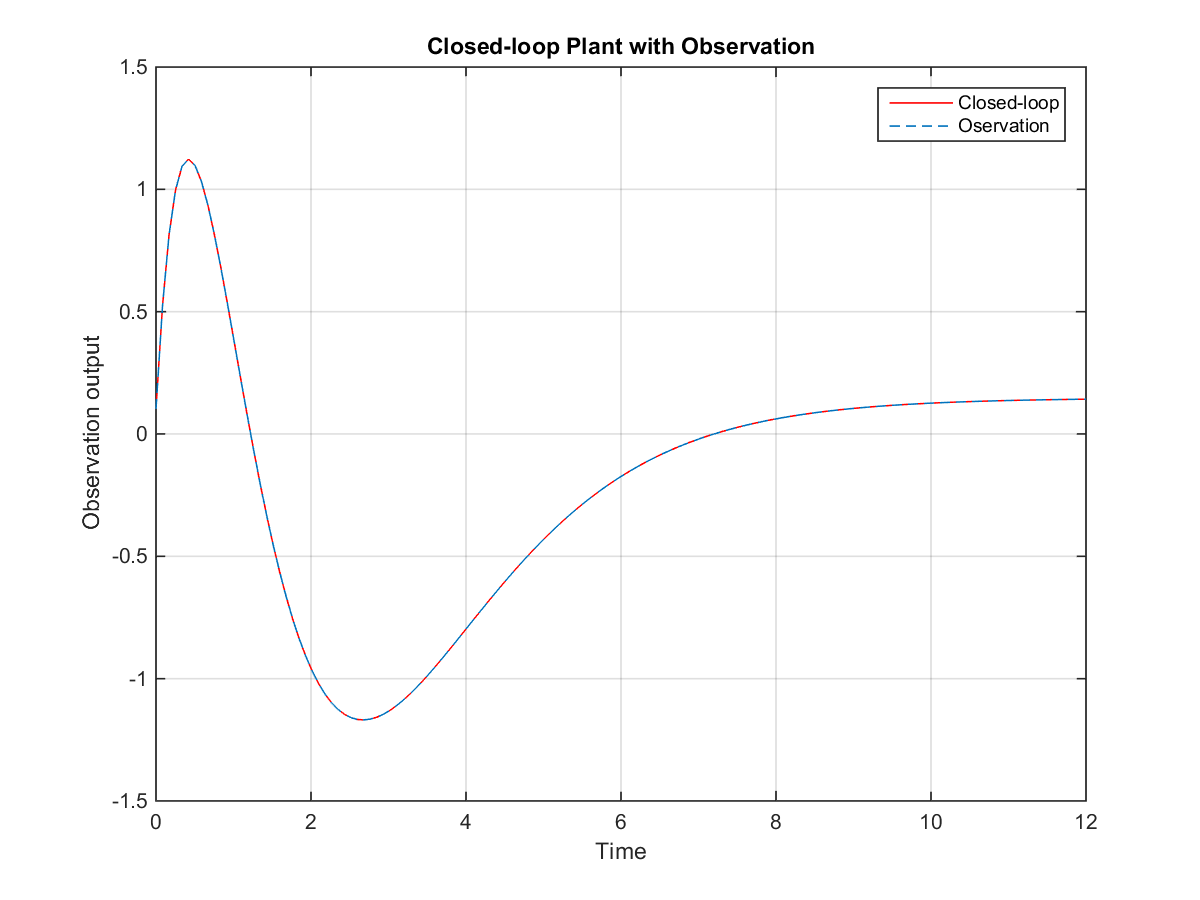
\includegraphics[scale = 0.55]{ClosedLoopObservation.png}
		\caption{Closed-loop with Observation in next 12 seconds}
		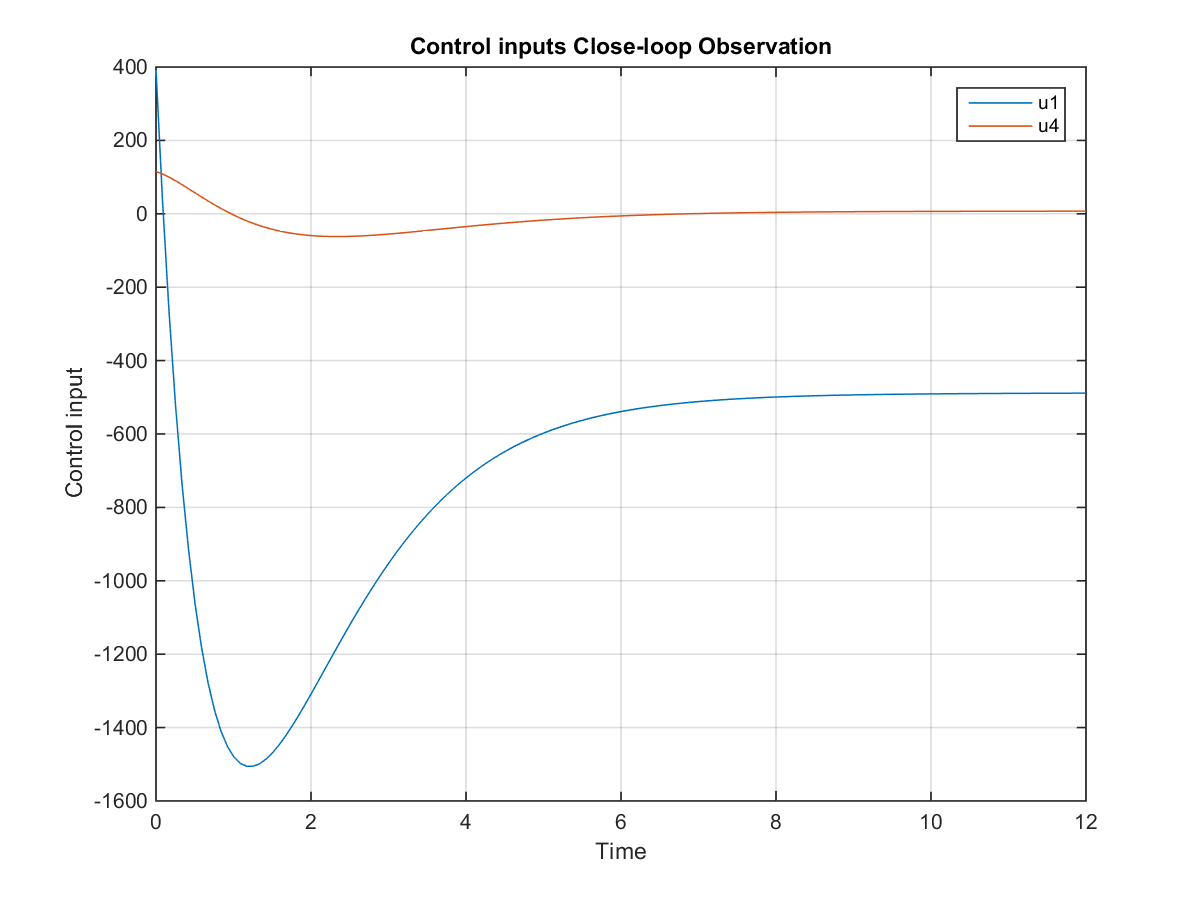
\includegraphics[scale = 0.55]{ClosedLoopControlInput.png}
		\caption{Closed-loop Control inputs with Observation in next 12 seconds}
	\end{center}
\end{figure} \\
\pagebreak

	Complete simulation for system in 16 seconds:
\begin{lstlisting}
%% Plot all system output and control input
yt = [yOp;yOC];
tt = [tOp;4+tOC];
figure;
plot(tt,yt(:,1),'r',tt,yt(:,2),'--'); grid on;
xlabel('Time'); ylabel('Output Y');
legend('Output','Observation');
title('Ouput Simulation System in 16 seconds');
print('OutputSimulation16s','-dpng');
\end{lstlisting}
\begin{figure}[htp]
	\begin{center}
		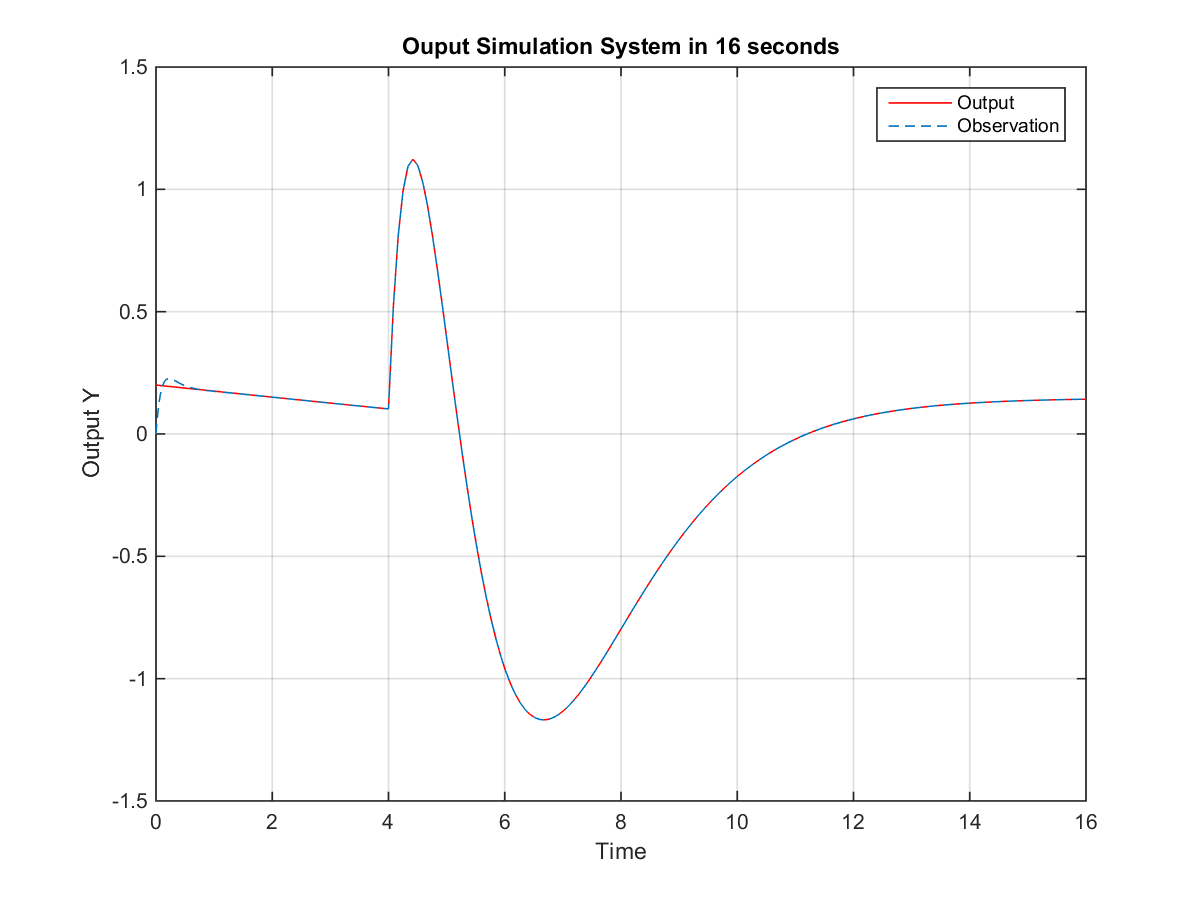
\includegraphics[scale = 0.9]{OutputSimulation16s.png}
		\caption{Output Simulation System in 16 seconds}
	\end{center}
\end{figure}

\begin{lstlisting}
u_temp = G2*sOp';
sizeUOp = size(u_temp);
UOp = zeros(sizeUOp);
ut = [UOp, UgC];
figure;
plot(tt,ut); grid on;
xlabel('Time'); ylabel('Control input');
legend('u1','u4');
title('Control inputs in Simulation system in 16 seconds');
print('ControlInputSimulation16s','-dpng');
\end{lstlisting}	
\begin{figure}[htp]
	\begin{center}
		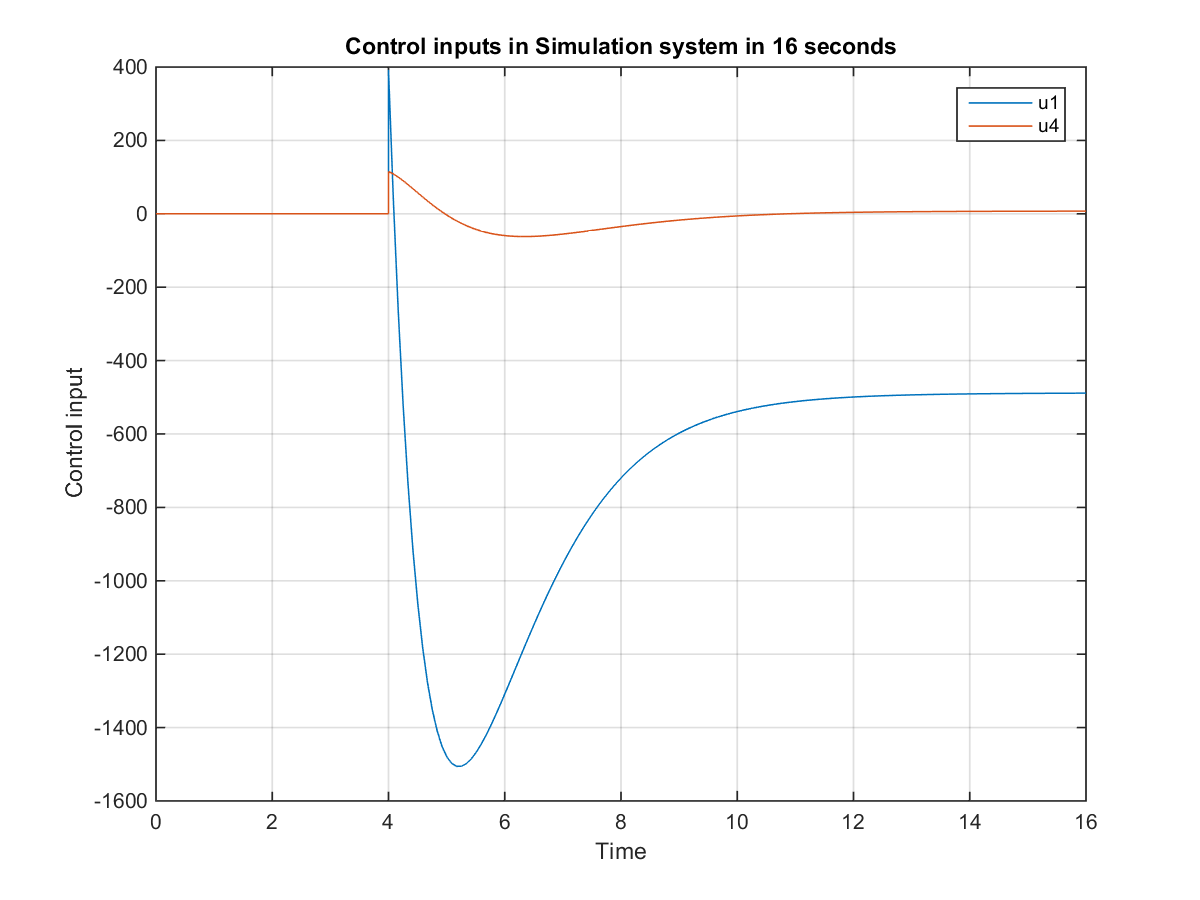
\includegraphics[scale = 0.9]{ControlInputSimulation16s.png}
		\caption{Control inputs in Simulation system in 16 seconds}
	\end{center}
\end{figure}	
\pagebreak
	
	Plot system: \\
\begin{figure}[htp]
	\begin{center}
		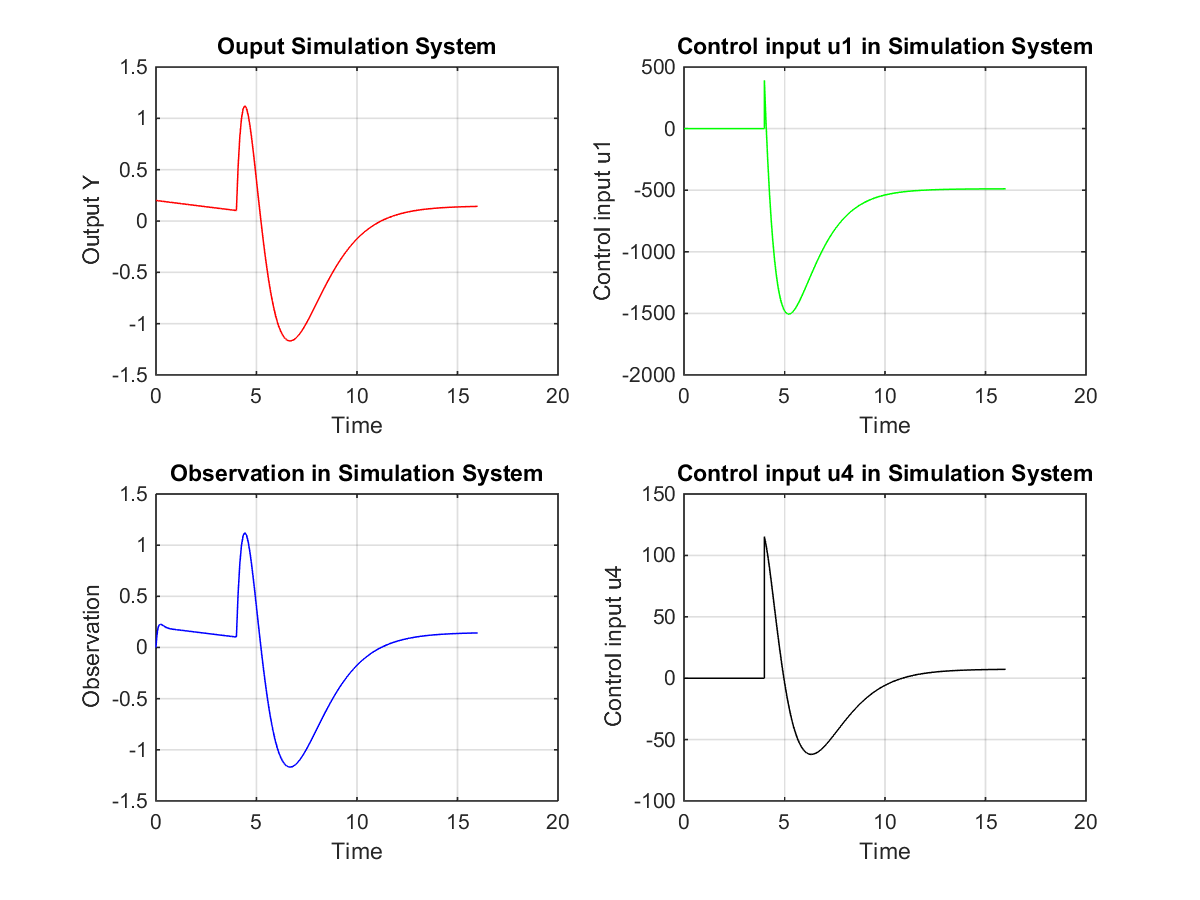
\includegraphics[scale = 0.9]{SimulationSystem.png}
		\caption{Full Simulation system in 16 seconds}
	\end{center}
\end{figure}		
	
	
\end{document}